%% Follow comments to support use.

%%%%%%%%%%%%%%%%%%%%%%%%%%%%%%%%%%%%%%%%%%%%%%%%%%%%%%%%%
%% STEP 1: Choose options for MSc / BSc / seminar layout and your bibliographic style
%%%%%%%%%%%%%%%%%%%%%%%%%%%%%%%%%%%%%%%%%%%%%%%%%%%%%%%%%

\documentclass[finnish,twoside,censored,tkt]{HYthesisML} 

% If wanted, open new chapters only at right page.
% By default, "openany".
%\PassOptionsToClass{openright,twoside,a4paper}{report}
\PassOptionsToClass{openany,twoside,a4paper}{report}

\usepackage{csquotes}
%%%%%%%%%%%%%%%%%%%%%%%%%%%%%%%%%%%%%%%%%%%%%%%%%%%%%%%%%
%% REFERENCES
%% Some notes on bibliography usage and options:
%% natbib -> you can use, e.g., \citep{} or \parencite{} for (Einstein, 1905); with APA \cite -> Einstein, 1905 without ()
%% maxcitenames=2 -> only 2 author names in text citations, if more -> et al. is used
%% maxbibnames=99 as no great need to suppress the biliography list in a thesis
%% for more information see biblatex package documentation, e.g., from https://ctan.org/pkg/biblatex 

%% Reference style: select one 
%% for APA = Harvard style = authoryear -> (Einstein, 1905) use:
%\usepackage[style=authoryear,bibstyle=authoryear,backend=biber,natbib=true,maxnames=99,maxcitenames=2,uniquelist=minyear,giveninits=true,uniquename=mininit]{biblatex}
%% for numeric = Vancouver style -> [1] use:
\usepackage[style=numeric,bibstyle=numeric,backend=biber,natbib=true,maxbibnames=99,giveninits=true,uniquename=init]{biblatex}
%% for alpahbetic -> [Ein05] use:
%\usepackage[style=alphabetic,bibstyle=alphabetic,backend=biber,natbib=true,maxbibnames=99,giveninits=true,uniquename=init]{biblatex}
%

\addbibresource{bibliography.bib}
% in case you want the final delimiter between authors & -> (Einstein & Zweistein, 1905) 
% \renewcommand{\finalnamedelim}{ \& }
% List the authors in the Bibilipgraphy as Lastname F, Familyname G,
\DeclareNameAlias{sortname}{family-given}
% remove the punctuation between author names in Bibliography 
%\renewcommand{\revsdnamepunct}{ }


%% Block of definitions for fonts and packages for picture management.
%% In some systems, the figure packages may not be happy together.
%% Choose the ones you need.

%\usepackage[utf8]{inputenc} % For UTF8 support, in some systems. Use UTF8 when saving your file.

\usepackage{lmodern}         % Font package, again in some systems.
\usepackage{textcomp}        % Package for special symbols
\usepackage[pdftex]{color, graphicx} % For pdf output and jpg/png graphics
\usepackage{epsfig}
\usepackage{subfigure}
\usepackage[pdftex, plainpages=false]{hyperref} % For hyperlinks and pdf metadata
\usepackage{fancyhdr}        % For nicer page headers
\usepackage{tikz}            % For making vector graphics (hard to learn but powerful)
%\usepackage{wrapfig}        % For nice text-wrapping figures (use at own discretion)
\usepackage{amsmath, amssymb} % For better math

\singlespacing               %line spacing options; normally use single

\fussy
%\sloppy                      % sloppy and fussy commands can be used to avoid overlong text lines
% if you want to see which lines are too long or have too little stuff, comment out the following lines
% \overfullrule=1mm
% to see more info in the detailed log about under/overfull boxes...
% \showboxbreadth=50 
% \showboxdepth=50



%%%%%%%%%%%%%%%%%%%%%%%%%%%%%%%%%%%%%%%%%%%%%%%%%%%%%%%%%
%% STEP 2:
%%%%%%%%%%%%%%%%%%%%%%%%%%%%%%%%%%%%%%%%%%%%%%%%%%%%%%%%%
%% Set up personal information for the title page and the abstract form.
\title{Ketterän ohjelmistokehitysryhmän hallinnalliset haasteet}
\author{Benjamin Blinnikka}
\date{\today}

% Set supervisors, use the titles according to the thesis language
\supervisors{FM Nea Pirttinen}
\examiners{TkT Emilia Oikarinen}

\keywords{ketterä, ohjelmistokehitys, kehitysryhmä, hallinta, haasteet}
\additionalinformation{\translate{\track}}

%% Provide classification terms, to appear on the abstract page.
\classification{\protect{\ \\
    Software and its engineering $\rightarrow$ 
    Software creation and management \\ $\rightarrow$ 
    Software development process management $\rightarrow$  
    Software development methods \\ $\rightarrow$ 
    Agile software development
}}

%% If you want to quote someone special. You can comment this line out and there will be nothing on the document.
%\quoting{Bachelor's degrees make pretty good placemats if you get them laminated.}{Jeph Jacques}


%% OPTIONAL STEP: Set up properties and metadata for the pdf file that pdfLaTeX makes.
\hypersetup{
    unicode=true,                                   % to show non-Latin characters in Acrobat’s bookmarks
    pdftoolbar=true,                                % show Acrobat’s toolbar?
    pdfmenubar=true,                                % show Acrobat’s menu?
    pdffitwindow=false,                             % window fit to page when opened
    pdfstartview={FitH},                            % fits the width of the page to the window
    pdftitle={Ketterän ohjelmistokehitysryhmän hallinnalliset haasteet},            % title
    pdfauthor={Benjamin Blinnikka},                                                 % author
    pdfsubject={Ketterän ohjelmistokehitysryhmän hallinnalliset haasteet},          % subject of the document
    pdfcreator={Benjamin Blinnikka},                % creator of the document
    pdfproducer={pdfLaTeX},                         % producer of the document
    pdfkeywords={ketterä} {ohjelmistokehitys} {kehitysryhmä} {hallinta} {haasteet}, % list of keywords for
    pdfnewwindow=true,                              % links in new window
    colorlinks=true,                                % false: boxed links; true: colored links
    linkcolor=black,                                % color of internal links
    citecolor=black,                                % color of links to bibliography
    filecolor=magenta,                              % color of file links
    urlcolor=cyan                                   % color of external links
}

%%-----------------------------------------------------------------------------------

\begin{document}

% Generate title page.
\maketitle

%%%%%%%%%%%%%%%%%%%%%%%%%%%%%%%%%%%%%%%%%%%%%%%%%%%%%%%%%
%% STEP 3:
%%%%%%%%%%%%%%%%%%%%%%%%%%%%%%%%%%%%%%%%%%%%%%%%%%%%%%%%%
%% Write your abstract in the separate file, to be positioned here.

% Tämä dokumentti on tarkoitettu Helsingin yliopiston tietojenkäsittelytieteen osaston opin\-näyt\-teiden ja harjoitustöiden ulkoasun ohjeeksi ja mallipohjaksi. Ohje soveltuu kanditutkielmiin, ohjelmistotuotantoprojekteihin, seminaareihin ja maisterintutkielmiin. Tämän ohjeen lisäksi on seurattava niitä ohjeita, jotka opastavat valitsemaan kuhunkin osioon tieteellisesti kiinnostavaa, syvällisesti pohdittua sisältöä.

% Työn aihe luokitellaan  
% ACM Computing Classification System (CCS) mukaisesti, 
% ks.\ \url{https://dl.acm.org/ccs}. 
% Käytä muutamaa termipolkua (1--3), jotka alkavat juuritermistä ja joissa polun tarkentuvat luokat erotetaan toisistaan oikealle osoittavalla nuolella.

\begin{abstract}

Tämä rakentuu tutkielman rakentumisen myötä.

\end{abstract}


% Place ToC
\mytableofcontents
\mainmatter

%%%%%%%%%%%%%%%%%%%%%%%%%%%%%%%%%%%%%%%%%%%%%%%%%%%%%%%%%
%% STEP 4: Write the thesis.
%%%%%%%%%%%%%%%%%%%%%%%%%%%%%%%%%%%%%%%%%%%%%%%%%%%%%%%%%
%% Your actual text starts here. You shouldn't mess with the code above the line except
%% to change the parameters. Removing the abstract and ToC commands will mess up stuff.
%%
%% Command \include{file} includes the file of name file.tex.
%% A new page will be created at every \include command, 
%% which makes it appropriate to use it for large entities such as book chapters. Cannot be nested.
%% It is useful for a big project, as changing one of the include targets 
%% won't force the regeneration of the outputs of all the rest.
%% Alternatively, \input is a more lower level macro 
%% which simply inputs the content of the given file like it was copy&pasted there manually.

\chapter{Johdanto\label{intro}}

Ketterä ohjelmistokehitys (jatkossa \textit{ketterä}) on suosittu kehitysaate nykypäivän ohjelmistokehityksessä, minkä avulla ohjelmistoja voidaan rakentaa ja muokata tehokkaasti asiakkaan tarpeiden ympärille. Ketterän suosio perustuu periaatteisiin, joiden myötä ohjelmistoprojektien onnistuvuusprosentin ja asiakastyytyväiseyyden on todettu nousevan \cite{9533020}. Ketterää toteutetaan niin sanotuilla ketterillä menetelmillä, joista yleisimpien joukkoon lukeutuvat esimerkiksi Scrum \cite{SCRUMORG} ja XP \cite{XPORG}. Ketterää on haluttu kehittää entisestään tutkimalla ja kartoittamalla yleisimpiä haasteita ja niiden syitä \cite{7872736}.

Tutkimuksessaan Fitriani et al. \cite{7872736} totesivat yleisimmäksi haastealueeksi ketterää käyttävässä ryhmässä (jatkossa \textit{ketterä ryhmä}) hallinnalliset haasteet jaetulla ilmaantuvuudella hajautettuihin ryhmiin liittyvissä haasteissa, mitkä itsessään liittyvät vahvasti ensimmäiseen. Tutkimus julkaistiin vuoden 2016 ICACSIS-konferenssissa tavoitteenaan tuoda esille ketterään liittyviä yleisiä haasteita. Tutkimuksessa koottiin yhteen 20 eri haasteita käsittelevää tutkimusta, joista ilmeni kaiken kaikkiaan 30 haastetta. Yhdeksässä tutkimuksista käsiteltiin ketterään ohjelmistokehitysryhmään liittyviä hallinnallisia haasteita, joita ovat muun muassa suunnitteluun, koordinointiin, käytökseen sekä ryhmän käytänteisiin liittyvät huomiot. Ketterän ryhmän hallinnalliset haasteet ovat merkittäviä johtuen ketteristä periaatteista, joiden myötä muun muassa yksilö ja vuorovaikutus asetetaan tärkeämmäksi suhteutettuna prosesseihin ja työkaluihin \cite{beck2001agile}. Periaatteen myötä ketterä ryhmä on lähtökohtaisesti toiminnassaan autonominen, jonka myötä ryhmän hallinta ja suunnan ohjaus tapahtuu ryhmän toimesta. Hallinnallisuuteen liittyvät haasteet ovat myös merkittäviä siksi, että aihealueen on todettu olevan suurin vaikuttava tekijä tuottavuuteen \cite{DEOMELO2013412}.

Ketteryyteen liittyvään autonomisuuteen liittyy sekä vapautta muotoilla sopivat työskentelytavat että riskejä syöstä projekti pahimmassa tapauksessa raiteiltaan. Ilman ammattitaitoista ja ketteriin periaatteisiin tutustunutta ryhmää ryhmän projektin ohjaus ja ryhmänhallinta voivat olla hyvinkin haastavia \cite{7872736}. Vaikka ketterässä on monia hyviä puolia niin ryhmädynamiikan kuin asiakkaan kannalta, ketterän ryhmän toimintaan liittyy lukuisia mahdollisia haasteita. Haasteita ilmenee esimerkiksi tapauksissa, joissa ketterää yritetään käyttää tai toteuttaa puutteellisesti. Yksi merkittävimmistä haasteiden lähteistä on asetelma, jossa ketterää toteutetaan ymmärtämättä sen ydinperiaatteita. Toinen yleinen lähde haasteille on tilanne, jossa ketterää menetelmää käytetään puuttellisesti, minkä myötä joistain käytetyn menetelmän käytänteistä luovutaan tai jätetään vähemmälle. Esimerkkinä tilanteesta toimii niin sanottu ScrumBut \cite{SCRUMBUT}, jossa ketterä ryhmä on ottanut käyttöön Scrumin, mutta eivät toteuta sitä käytänteiltään täysimittaisesti esimerkiksi viikottaisten tapaamisten tai retrospektiivien suhteen.

Edellä pohditut skenaariot johtavat suuremmalla todennäköisyydellä haasteisiin ketterässä ryhmässä ja projektissa, minkä myötä projektin ja ketterän ryhmän hallinnasta voi tulla hyvinkin haastavaa. Haasteita käsiteltäessä on syytä huomioida ketterien ryhmien eri ryhmäkoot. Haasteet voivat esiintyä minkä kokoisessa ryhmässä tahansa niiden perustuessa samaan aatteeseen, mutta niiden voidaan olettaa muodostavan suurempaa riskiä ja potentiaalista vahinkoa suuremmissa variaatioissa, kuten maailmanlaajuisesti hajautetussa ketterässä kehityksessä \cite{ALZOUBI201622}. Tulevat kappaleet toimivat yleisimpien haastealueiden ja niihin liittyvien haasteiden esittelijöinä ja käsittelijöinä. Tietenkin on huomioimisen arvoista, että haasteet voivat mennä useamman kuin yhden kategorian alle, minkä myötä haastealueisiin jako ei ole täysin poissulkevaa. Tässä tutkielmassa keskitytään pohtimaan seuraavia kysymyksiä: \begin{enumerate}
    \item Mitä hallinnallisia haasteita liittyy ketterään ryhmään?
    \item Mitä ratkaisumalleja on olemassa ketterän ryhmän hallinnallisiin haasteisiin?
\end{enumerate}

\chapter{Koordinaatio}

\begin{figure}[t]
\centering 
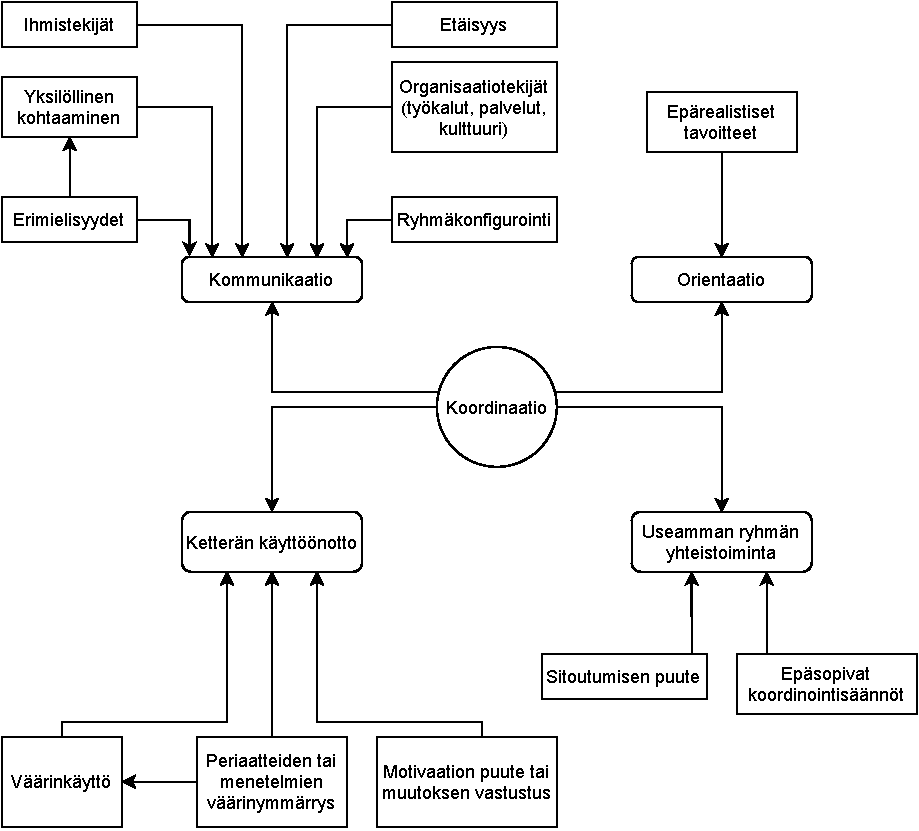
\includegraphics[width=0.9\textwidth]{template/figures/koordinaatiohaasteet.pdf}
\caption{Kaavio koordinaatiohaasteista ja niiden tekijöistä perustuen Alzoubi et al. \cite{ALZOUBI201622}, de Melo et al. \cite{DEOMELO2013412}, Gregory et al. \cite{GREGORY201692}, Moe et al. \cite{MOE2012853} ja Silva et al. \cite{SELLERISILVA201520} tutkimuksiin.\label{fig:koordinaatiohaasteet}}
\end{figure}

Koordinaatiota voidaan tarkastella suurimpana vaikuttavana alueena ketterää ohjelmistokehitystä noudattavassa ryhmässä. Aihetta voidaan ajatella koko toimintaketjun sitovana liimana, sillä valtaosan esitettävistä aihealueista voidaan tulkita kuuluvan koordinaation alle. Tämä tutkielma jaottelee ryhmän koordinaatiohaasteet ketterän käyttöönottoon, kommunikaatioon, useamman ryhmän väliseen koordinaatioon sekä orientaatioon. Koordinaatio aiheena kattaa kaiken, joka voidaan tulkita vaikuttavan kehitysryhmän sisäiseen tai ulkoiseen yhteistoimintaan. Ryhmän sisäiseksi koordinaatioksi tulkitaan tässä kontekstissa ryhmäläisten välinen interaktio, kun taas ulkoiseksi koordinaatioksi tulkitaan esimerkiksi organisaation puolelta tuleva ohjeistaminen (tai ohjaus), mahdollisten muiden saman projektin parissa työskentelevien ryhmien kanssa yhteistyöskentely ja asiakkaan kanssa toimiminen. Esimerkkitapaus ulkoisesta koordinaatiosta on projekti, joka toteutetaan maailmanlaajuisesti hajautetulla ketteränä ohjelmistokehityksenä \cite{ALZOUBI201622}. Esitettävät haasteet voidaan tulkita vaikuttavan voimakkaammin niin laajemmissa ja maailmanlaajuisesti hajautetuissa ketterän kehityksen ryhmissä verrattuna niin sanotusti paikalliseen ryhmään. Maailmanlaajuisesti hajautettu ketterä kehitys tarkoittaa sitä, että prosessi koostuu ryhmistä tai ryhmäläisistä, jotka sijaitsevat maantieteellisesti kaukana toisistaan. Paikallinen ketterä kehitys tarkoittaa tässä kontekstissa vastakohtaa. Koordinaation ollessa laaja käsite, siihen on yhdistettävissä lukuisia mahdollisia haasteita aina yhteistoiminnan käyttöönotosta ylläpitoon. Tulevissa alakappaleissa tutkielma esittelee kuvan \ref{fig:koordinaatiohaasteet} mukaisesti yleisimmät koordinaatiohaasteet, niiden tekijöitä ja vaikutuksia sekä mahdollisia ratkaisumalleja.

\section{Ketterän käyttöönotto}

Ensimmäisenä haasteena ketterän koordinointiin liittyen on ketterän menetelmän käyttöönotto ja siispä ketteriä periaatteita noudattavan ryhmän luonti. Eräänä haasteena käyttöönottoon liittyen on todettu tilanne, jossa perinteisiä malleja, kuten vesiputousta harjoittanut organisaatio haluaa ketteryyttä pohjautuen tietoon, että ketterä tuottaa parempaa kilpailukykyä \cite{MCKNIGHT2014168}. Haasteita tässä tapauksessa voi tuottaa organisaation ymmärrystaso ketteristä periaatteista ja niiden toteutustavoista. Puutteellinen ymmärrys voi olla seuraamusta käyttöönottoon liittyvästä puutteellisesta motivaatiosta, joka juontaa juurensa menetelmätottumuksiin \cite{GREGORY201692}. Syynä voi olla myös muutoksen vastustus tai liian haastelähtöinen näkökulma ketterään kehitykseen, kuten \cite{SELLERISILVA201520} toteavat. Mikäli organisaatiossa ei ymmärretä ketteryyteen liittyviä hyötyjä, siihen liittyviä riskejä tai varsinaisia toteutusmenetelmiä on odotettavissa haastava tie käyttöönoton suhteen.

Tutkimuksessaan Gregory et al. \cite{GREGORY201692} toteavat haasteita ketterän toteuttamiseen ja käyttöönottoon liittyen perinteisen ympäristön ja organisaation kontekstissa. Eräänä rajoittavana tekijänä käyttöönottoon liittyen todettiin ketterän väärinkäyttö, joka johtuu väärinymmärryksestä. Tutkimuksessa ilmeni tilanne väärinkäytöstä, missä organisaation johto on teettänyt ketterän ryhmän työskentelemään massiivisen määrän ylitöitä perustellen sen olevan osana ketteryyttä. Skenaariossa on nähtävissä kehittäjien loppuunpalaminen sekä organisaation paluu perinteisten menetelmien käyttöön, kun uusi menetelmä ei olekaan tuottanut odotettua tulosta. Toisena väärinkäyttöön liittyvänä skenaariona ilmeni tilanne, jossa jonkin ketterän menetelmän käyttöönoton jälkeen organisaation johto on mikromanageroinut kehitysryhmää ainakin siihen saakka, kunnes nähtävää tulosta on alkanut muodostumaan. Jatkuvan mikromanageroinnin seurauksena on nähtävissä varsinaisen ketteryyden ja sen sisältävän luovuuden väheneminen. Toisaalta ohjaukseen liittyen Silva et al. \cite{SELLERISILVA201520} toteavat olevan oleellista tukea ja ohjata ketterän käyttöönottoa aikaisissa vaiheissa.

Käyttöönottohaasteiden minimoimiseksi on todettu olevan suositeltavaa hakea konsultointia ammattilaisilta ja yrityksiltä, joilla on erityisosaamista ketterään kehitykseen liittyen \cite{SELLERISILVA201520}. Silva et al. \cite{SELLERISILVA201520} muistuttavat lisäksi, että ketterien periaatteiden mukaisesti ketterän kehitysryhmän tulisi pyrkiä itse esittämään ratkaisumalleja ongelmatilanteisiin.

\section{Kommunikaatio}

Kommunikaation voidaan ajatella olevan ketterän ryhmän koordinaation mahdollistava työkalu. Ilman kommunikaatiota ei olisi yhteistoimintaa, ainakaan tehokkaanlaatuista. Alzoubi et al. \cite{ALZOUBI201622} korostavat kommunikaation tehokasta käyttöönottoa alusta alkaen muiden haasteiden välttämiseksi. Haasteiden minimoimiseksi olisi olennaista, että ketterä ryhmä kommunikoi ryhmäläistensä kesken ja ryhmän ulkopuolella olevien yhteistyötahojen kanssa. Kommunikaation merkitys korostuu maantieteellisesti hajautettujen ryhmien osalta, sillä kyseiset kehittäjät eivät lähtökohtaisesti pääse samaan työskentelytilaan muiden kanssa. Ketterien periaatteiden korostaessa asiakasyhteistyötä on myös ratkaisevaa, että ryhmä kommunikoi asiakkaan kanssa riittävän selkeästi ja usein.

Tutkimuksessaan Alzoubi et al. \cite{ALZOUBI201622} keskittyvät ketterään liittyvään kommunikaatioon ja tuovat esille siihen liittyviä haasteita ja ratkaisumalleja. Tutkimus itsessään keskittyy maailmanlaajuisesti hajautetun ketterän ohjelmistokehityksen kommunikatiivisiin seikkoihin, mutta tuloksia voidaan soveltaa paikallisesti toteutettavaan variaatioon oletuksella, että paikallisvariaatiossa haasteet ovat lievempiä. Tutkimuksessa puutteellisen kommunikoinnin todettiin johtavan kaikkiin muihin haasteisiin ja niiden käsittelyn vaativan 2,5 kertaa enemmän resursseja kuin paikallisessa variaatiossa. Alzoubi et al. toteavat ketterän kehityksen nojaavan epävirallisiin kommunikointikeinoihin ryhmäläisten välillä, sillä kommunikoinnin on todettu olevan huomattavasti tehokkaampaa epävirallisten menetelmien pohjalta. Epäviralliset kommunikointimenetelmät voidaan jakaa henkilökohtaiseen, vuorovaikutteiseen ja vertaisorientoituneeseen tapaan. Epävirallisen kommunikoinnin on todettu nojaavan voimakkaasti vuorovaikutukseen, joka tapahtuu kasvotusten niin ryhmäläisten kuin ryhmän ja asiakkaan välillä. Tästä johtuen ryhmäläisten välinen sijainti korostuu voimakkaasti vaikuttavana tekijänä.

Alzoubi et al. tutkimuksessa \cite{ALZOUBI201622} todettiin, että lähteinä kommunikointihaasteille ovat muun muassa etäisyys, organisaatiotekijät, ihmistekijät ja ryhmäkonfigurointi. Etäisyyden todettiin olevan yleisin haasteiden lähde. Sen todettiin hankaloittavan koordinaatiota esimerkiksi viiveinä kommunikoinnissa, pidempinä kokouksina, hankaluutena löytää yhteisiä työaikoja ja luottamuksen puutteena. Silva et al. tutkimuksessa \cite{SELLERISILVA201520} rajoittavana tekijänä todettiin ryhmän sisäiset erimielisyydet, joiden voidaan olettaa hankaloittavan kommunikointia. Ryhmäkonfigurointiin liittyen sekä \cite{SELLERISILVA201520} että \cite{ALZOUBI201622} toteavat kommunikoinnin hankaloituvan sen mukaan, mitä suurempi ryhmä on kyseessä. Sama pätee myös tapaukseen, jossa projektin parissa työskentelee useampi ryhmä. Lisäksi Alzoubi et al. \cite{ALZOUBI201622} toteavat, että satunnaisissa tapauksissa jotkin ryhmäläiset eivät halua kommunikoida ja omaavat huonomman ymmärryksen koordinaatiosta. Kommunikoinnin haluttomuuteen liittyy myös Moe et al. \cite{MOE2012853} tutkimus, jossa haasteena todetaan ryhmäläisten keskinäinen kohtaaminen. Ryhmäläiset eivät välttämättä halua väitellä keskenään, vaan mieluummin mukautuvat tilanteeseen. Seurauksena haasteista ryhmäkonfiguraatiossa on muun muassa aikaisen vaiheen kommunikointiongelmat, ryhmäläisten haluttomuus ryhmäkommunikointiin, vähentynyt ymmärrys ryhmätyöskentelystä sekä hitaus kommunikoinnissa \cite{ALZOUBI201622}. Lisäksi keskinäisen kohtaamattomuuden seurauksena on ryhmän tehoton päätöksenteko \cite{MOE2012853}. Organisaatiotekijöiksi listattiin organisaation työkalut ja palveluiden kyky tukea kommunikointia \cite{ALZOUBI201622}. Työkaluihin ja palveluihin lukeutuvat muun muassa puhelin, pikaviestipalvelut sekä sähköposti. Merkittäväksi tekijäksi on listattu myös organisaation kulttuuri, joka koostuu asenteista, arvoista ja käytänteistä. Seurauksena organisaatiotekijöistä ovat muun muassa tehottomampi ryhmä, huonolaatuisempi ohjelmisto, suurempi määrä työkaluja sekä puutteellinen luotto.

Ratkaisumalleiksi Alzoubi et al. \cite{ALZOUBI201622} listaavat seuraavanlaista. Ryhmäkonfiguraatiosta lähtöisin oleviin haasteisiin ehdotetaan strategiaksi ensinnäkin paikallisten tapaamisten järjestämistä. Paikallisten tapaamisten on todettu tuottavan epävirallisempaa kommunikointia, joka tehostaa ryhmän tuottavuutta \cite{DEOMELO2013412}. Toisaalta \cite{ALZOUBI201622} listaavat samalla osaksi strategiaa tehokkaan virallisen kommunikoinnin lisäämisen. Muita osia strategiasta ovat muun muassa projektin säännöllinen esittely osapuolille, säännöllisten tapaamisten järjestäminen, paikallisten ryhmien muodostus sekä selkeiden roolien ja vastuiden jako. Toisaalta \cite{CLAPS201521} toteavat roolien jakoon liittyen erittäin oleelliseksi oikeanlaisen ohjauksen mahdollisen johdon puolelta, ettei prosessi ole vahingollinen ryhmille. Claps et al. \cite{CLAPS201521} korostavat roolijaon olevan itsessään haastava tehtävä. Organisaatiotekijöistä lähtöisin oleviin haasteisiin Alzoubi et al. \cite{ALZOUBI201622} ehdottavat strategiaksi korostaa työskentelykulttuuria, joka suosii jatkuvaa kommunikointia, luottoa sidosryhmien välillä sekä nopeaa asiakaspalautetta. 

\section{Useamman ryhmän yhteistoiminta}

Tutkimuksessaan de Melo et al. \cite{DEOMELO2013412} toteavat ketterän ryhmän tuottavuuden koostuvan ryhmän sisäisistä ja ulkoisista tekijöistä. Ryhmän ulkoiset tekijät rajautuvat useamman ryhmän väliseen koordinaatioon. On todettu, että useista kehitysryhmistä koostuvien projektien ryhmien välinen koordinaatio on yksi hankalimmista kehitettävistä asioista ohjelmistotuotantoon liittyen. Ryhmien välisen koordinoinnin haasteita aiheuttavat sitoutumisen puute sekä epäsopivat koordinointisäännöt ryhmien välillä. Haasteiden on todettu aiheuttavan suuntausvirheitä ja ketteryyden rikkoutumisen. Esimerkkinä suuntausvirheestä toimii tilanne, jossa ryhmän työskentely riippuu toisen ryhmän tuloksista, eivätkä ryhmät työskentele samassa tahdissa. Tällöin syntyy tilanteita, joissa toisesta ryhmästä riippuva ryhmä joutuu odottamaan tai hidastamaan tahtiaan merkittävästi. Toisesta ryhmästä riippuvuuden on todettu olevan yleinen ilmiö laajemmissa ohjelmistoprojekteissa.

Laajojen, useista kehittäjäryhmistä koostuvien projektien osalta on todettu olevan haastavaa toteuttaa laaja-alaista ketterää kehitystä \cite{DEOMELO2013412}. Kaikki ryhmät eivät välttämättä noudata ketteriä periaatteita tai käytä mitään ketterää menetelmää. De Melo et al. \cite{DEOMELO2013412} toteavat, että ketterän ryhmän on äärimmäisen hankalaa tai jopa mahdotonta vaikuttaa muiden ryhmien työskentelymenetelmiin. Täten tilanne, jossa osa ryhmistä käyttää eri ketteriä menetelmiä ja osa vesiputousmallia, on mahdollinen. Projektin useat eri kehitysmenetelmät voivat aiheuttaa massiivisia koordinointiongelmia. De Melo et al. mainitsevat ratkaisuna useamman ryhmän yhteistoimintaan ketterän ryhmän kyvyn mukautua erilaisiin tilanteisiin. Mukautumisen kautta voisi olla mahdollista löytää paremmin yhteisiä työskentelytapoja eri menetelmiä käyttävien ryhmien kanssa erityisesti tilanteessa, jossa kumpikin (tai useampi) osapuoli noudattaa jotain ketterää menetelmää. Claps et al. \cite{CLAPS201521} mainitsevat, ettei ryhmien välinen koordinaatio olisi toiminut uuden ketterän menetelmän käyttöönoton kontekstissa ilman johdon käyttöönottamaa strategiaa. Organisaation johdon selkeän strategian myötä kullekin ryhmälle saatiin yhteinen tavoite, jonka myötä ryhmät työskentelivät samaa päämäärää kohti.

\section{Orientaatio}

Tutkimuksessaan Moe et al. \cite{MOE2012853} toteavat yhtenä koordinaatiohaasteena ryhmäorientaation puutteen. Ryhmäorientaatio tarkoittaa ryhmän yhteistä suuntaa ja sen toteuttaminen tarkoittaa sitä, että kukin ryhmässä työskentelee yhteistä päämäärää kohti. Tutkimuksen mukaan joissain tilanteissa ketterän ryhmän orientaatio voi olla alhainen epärealististen tavoitteiden takia. Alhaisen ryhmäorientaation myötä on todettu tapauksia, joissa yksittäiset ryhmäläiset tekevät omia päätöksiä projektin suhteen sen sijaan, että päätöksiä tehtäisiin yhdessä. Lisäksi ongelmaraportoinnin on todettu jäävän vähemmälle johtuen siitä, että alhaisen orientaation myötä projektiin liittyviä ongelmia pidetään enemmän henkilökohtaisina kuin ryhmän yhteisinä ongelmina. Kaiken kaikkiaan alhainen ryhmäorientaatio vähentää ryhmän kommunikointia merkittävästi ja sen voidaan tulkita lisäävän riskiä ryhmäläisten siiloutumiselle. Siiloutumisella tarkoitetaan sitä, että jokin osa ryhmästä alkaa työskentelemään suljetusti ilman muuta osaa ryhmästä.

\chapter{Kokoonpano}

Toisena merkittävänä alueena ketterän ryhmän hallinnallisissa haasteissa on ryhmäkokoonpanoon liittyvät haasteet, kuten muutokset ryhmässä ja kokoonpanon suunnittelu. Suunnittelun merkitys korostuu kokoonpanoon liittyvissä tehtävissä, kuten vastuunjaossa. On kuitenkin huomioitavaa, että suunnittelun merkitys nykyaikaisessa ohjelmistokehityksessä on muuttunut luonteeltaan perinteisiin malleihin, kuten vesiputousmalliin, nähden. Toisaalta puutteet suunnittelussa on kuitenkin yksi yleisimmistä ketterää toteuttavan ryhmän hallinnallisten haasteiden lähteistä \cite{7872736}. Beck et al. \cite{beck2001agile} määrittävät yhtenä ketteristä periaatteista, että muutokseen reagointi on tärkeämpää kuin suunnitelmassa pysyminen. Suunnitteluun liittyvät haasteet voidaan jakaa karkeasti ryhmäkokoonpanon ja ryhmien välisen koordinoinnin suunnitteluun, jotka itsessään jakautuu de Melo et al. \cite{DEOMELO2013412} mukaisesti ryhmän sisäisiin ja ulkoisiin tekijöihin.

\begin{figure}[t] % remove [h!] for automatic placement, which is probably better for a thesis with more text on page
\centering 
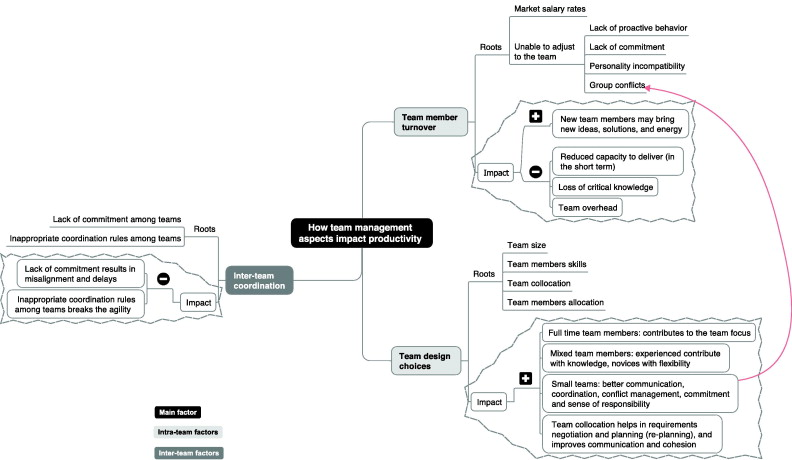
\includegraphics[width=1.0\textwidth]{template/figures/demelo.JPG}
\caption{De Melo et al. \cite{DEOMELO2013412} kaavio ketterän ryhmän tuottavuudesta.\label{fig:demelo}}
\end{figure}

\section{Ryhmäkokoonpano}

Tutkimuksessaan de Melo et al. \cite{DEOMELO2013412} toteavat ketterän ryhmän hallinnan olevan suurin vaikuttava tekijä tuottavuuteen. Tutkimus kartoitti merkittävimmät tuottavuuteen vaikuttavat tekijät, minkä myötä ne rajattiin ketterän ryhmän sisäisiin ja ulkoisiin haasteisiin. Ryhmän sisäisistä haasteista merkittävimmiksi korostuivat ryhmän suunnitteluvalinnat sekä jäsenten vaihtuvuus, kun taas ulkoisista haasteista merkittävimmäksi muodostui ryhmien välinen koordinaatio.

[\textbf{Katso löytyisikö seuraavaan kohtaan jotain lähteitä tukemaan vielä olettamusväitteitä, jotta olisi suorempaa viitettä}]


\section{Suunnitteluvalinnat}

[\textbf{Lisää Clapsin team role -pöhinät tänne!}]

Ryhmän suunnitteluvalinnat koostuvat tutkimuksessa \cite{DEOMELO2013412} ryhmäkoosta, ryhmäläisten taidoista, ryhmäläisten keskinäisestä sijainnista sekä ryhmäläisten jaosta. Tutkimuksesta on tulkittavissa, että haasteita kokoonpanoon tuottaa tässä kontekstissa muun muassa seuraavanlaiset tilanteet. Kokoonpanossa, jossa valtaosa ryhmäläisistä olisi osa-aikaisia työntekijöitä keskinäinen keskittyminen projektiin voisi olla heikkoa perustuen tutkimuksen toteamukseen tapauksesta, jossa täyspäiväjäsenillä on parempi keskittyminen. Ryhmän monipuolisuus kokemusten ja taitojen osalta on todettu hyödylliseksi siten, että kokeneilla on laaja kokemuskirjo, kun taas vähemmän kokeneet ryhmäläiset ovat yleensä joustavampia. Ryhmän kokoon liittyen on todettu, että pienemmän ryhmän koordinaatio (erityisesti kommunikoinnin osalta), konfliktinhallinta, sitoutuminen sekä vastuuntunto ovat paremmalla tasolla kuin suuremmissa ryhmissä. Ryhmän sijainnin on todettu vaikuttavan erityisesti vaatimusmäärittelyn ja suunnittelun toteutukseen siten, että paikallisessa ketterässä ryhmässä ne ovat huomattavasti helpompia. Paikallisen ryhmän kommunikointi sekä koheesio ovat myös parempia kuin esimerkiksi maantieteellisesti hajautetussa ryhmässä.

\section{Vaihtuvuus}

Ryhmän jäsenten vaihtuvuus on toinen ryhmän sisäistä haasteista. Vaihtuvuudeksi de Melo et al. \cite{DEOMELO2013412} määrittävät sekä aiemman kehittäjän lähtönä ryhmästä että uuden kehittäjän liittymisenä ryhmään. Vaihtuvuus aiheuttaa organisaatiolle monenlaisia kustannuksia, kuten irtisanoutumiseen, rekrytointiin sekä perehdyttämiseen liittyen. Lisäksi kehitysryhmä työskentelee vaihtuvuuden aikana astetta pienemmällä teholla johtuen joko pienemmästä määrästä kehittäjiä ryhmässä tai uuden ryhmäläisen perehdyttämisestä. Eräässä tutkimuksen tapauksista uusi ryhmäläinen  Tutkimuksessaan de Melo et al. määrittävät vaihtuvuuden tekijöiksi palkkatason sekä kehittäjän sopeutumattomuutena ryhmään. Sopeutumattomuuden on arvioitu johtuvan muun muassa oma-aloitteisuuden ja sitoutumisen puutteesta, epäsopivasta personaallisuudesta sekä ryhmän sisäisistä konflikteista. Viimeisestä on tulkittavissa, että haasteet kommunikoinnissa voivat aiheuttaa suunnitelmallisia haasteita. 

Vaikka vaihtuvuuden on todettu aiheuttavan suunnitelmallisia haasteita, niin sen on todettu myös vaikuttavan positiviisesti uusien ryhmäläisten kautta \cite{DEOMELO2013412}. On todettu, että uudet ryhmäläiset saattavat tuoda uusia ideoita, ratkaisuja ja yleisesti ottaen energiaa ryhmään. Toisaalta vaihtuvuuden negatiivisia vaikutuksia on lukumäärällisesti enemmän ja ne voidaan jakaa pidentyneeksi tuotantoajaksi lyhyellä aikavälillä, oleellisen tiedon menettämisenä poistumisen yhteydessä sekä lisäkustannuksina. 

De Melo et al. \cite{DEOMELO2013412} kiteyttävät ketterän ryhmän perustuvan yksilöihin ja ryhmätyöskentelyyn. Oikeilla menetelmillä toteutettuna kommunikaation ja yhteistyöskentelyn on todettu parantuvan. Lisäksi tutkimus korostaa ketterien menetelmien tehostavia työskentelytapoja, kuten pariohjelmointia, päivittäistapaamisten ja yhteisistuntojen pitämistä. Kaiken kaikkiaan ketterien menetelmien oikeanlaisen ja tarpeeksi laajan toteutuksen on todettu vähentävän vaihtuvuuden riskiä huomioiden vaihtuvuuden olevan varsin yleistä.

\section{Useamman ryhmän yhteistoiminta}

Tutkimuksessaan de Melo et al. \cite{DEOMELO2013412} toteavat ketterän ryhmän tuottavuuden koostuvan ryhmän sisäisistä ja ulkoisista tekijöistä. Ryhmän ulkoiset tekijät rajautuvat useamman ryhmän väliseen koordinaatioon ja sen suunnitteluun. Ryhmien välisen koordinoinnin haasteita aiheuttavat sitoutumisen puute sekä epäsopivat koordinointisäännöt ryhmien välillä. Haasteiden on todettu aiheuttavan suuntausvirheitä ja pahimmillaan ketteryyden rikkoutumisen. 
\chapter{Tutkielman, haasteiden ja ratkaisumallien arviointia}

Tässä kappaleessa tutkielma keskittyy arvioimaan omaa validiteettiaan ja reliabiliteettiaan sekä vertailemaan esitettyjä haastealueita ja niihin liittyviä mahdollisesti esitettyjä ratkaisumalleja. Tutkielman validiteetilla tarkoitetaan sitä, että arvioidaan kykeneekö tutkielma vastaamaan asetettuihin tutkimuskysymyksiin. Reliabiliteetilla tarkoitetaan sitä, että arvioidaan onko tutkielma luotettava ja tarkasteleeko se asioita esimerkiksi tarpeeksi objektiivisesti.

\section{Yleisesti}

Tutkielma jakoi haastealueet koordinaatioon ja kokoonpanoon pohjautuen Fitriani et al. \cite{7872736} tutkimukseen. Fitriani et al. tutkimus määritti hallinnallisiin haasteisiin kuuluvan kaikki ryhmän suunnitteluvalintoihin, koordinaatioon, käytökseen sekä ryhmän muihin käytänteisiin liittyvät haasteet. Tässä tutkielmassa haasteet rajattiin kahteen aihealueeseen: koordinaatioon ja kokoonpanoon. Kolmantena aihealueena olisi voinut olla yksilömuuttujiin pureutuva kappale, sillä useammassa tutkimuksessa ilmeni yksilön haasteiden vaikutus ryhmän hallintaan. Yksilömuuttujiin pureutuva kappale jätettiin pois sen keskittyessä enemmän yksilöön ja psykologiaan enemmän kuin varsinaiseen ryhmään. Tässä tutkielmassa ilmenevästä haastealueiden jaosta kahteen aiheeseen on syytä huomioida, että jako ei ole poissulkeva. Koordinaation tarkoittaessa kaikkea yhteistoimintaa mahdollistavaa, aiheen alle voi tulkita näkökulmasta riippuen melkein mitä vain. Voitaisiin esimerkiksi väittää, että tutkielman kolmas kappale, joka pureutuu kokoonpanohaasteisiin, lukeutuisi koordinaatioon, sillä ryhmäkokoonpano vaikuttaa huomattavasti ryhmän yhteistoimintaan. Edeltävänkaltaiset argumentit tiedostaen tutkielma ilmaisee jaon olevan karkea, eikä poissulje haasteiden kuuluvuutta useampaan kuin yhteen alueeseen. Lisäksi on huomioitavaa, että tämä tutkielma listaa vain yleisimmät haasteet rajallisesta määrästä lähteitä huomioiden, että kyseessä on varsin lyhyt kanditutkielma. Vielä lisäksi on huomioimisen arvoista, että haasteiden määrittelyyn käytetyt lähteet ovat jo usean vuoden vanhoja niiden ollessa keskimäärin vuosilta 2015 ja 2016. Tämän pohjalta tässä tutkielmassa ei välttämättä käsitellä sellaista oleelliseksi tulkittavaa tietoa niin haasteisiin kuin ratkaisuihinkaan liittyen, mikäli niihin liittyvä tieto on julkaistu lähivuosina.

\section{Haastealueet}

Tutkielman haastealueet jakautuvat ryhmän koordinaatioon ja kokoonpanoon. Koordinaatioon liittyvä kappale käsittelee yleisimmiksi ilmenneitä ryhmän (tai ryhmien) yhteistoimintaan vaikuttavia haasteita, kun taas kokoonpanoon liittyvä kappale käsittelee yleisimpiä ryhmäkokoonpanoon liittyviä haasteita. 

Kuvan \ref{fig:koordinaatiohaasteet} mukaisesti koordinaatiohaasteiksi määriteltiin ketterän käyttöönotto, ryhmän kommunikointi, useamman ryhmän välinen koordinaatio sekä ryhmäsuuntautumisen puute. Käyttöönottohaasteeseen liittyy tekijöinä ryhmän sisällä ilmenevä muutoksen vastustus, ketterien periaatteiden tai menetelmien väärinymmärrys sekä väärinkäyttö. Ketterien periaatteiden väärinymmärryksen todettiin johtavan väärinkäyttöön. Kommunikaation yhteyteen liittyy tekijöinä ryhmän erimielisyydet, yksilöllisen kohtaamisen puute, ihmistekijät, ryhmäläisten keskinäinen etäisyys, organisaatiotekijät sekä ryhmäkonfigurointi. Lisäksi erimielisyyksien todettiin johtavan yksilöllisen kohtaamisen haasteisiin. Useamman ryhmän väliseen koordinaatioon liittyen tekijöiksi todettiin ryhmäläisten (tai ryhmien) sitoutumisen puute sekä epäsopivat koordinointisäännöt. Lopulta orientaatiohaasteen ainoaksi tekijäksi todettiin ryhmän epärealistiset tavoitteet.

Kuvan \ref{fig:kokoonpanohaasteet} mukaisesti kokoonpanohaasteiksi lueteltiin ryhmän suunnitteluvalinnat sekä ryhmäläisten vaihtuvuus. Suunnitteluvalintaan todettiin vaikuttavan ryhmän koko, ryhmäläisten taidot, ryhmäläisten keskinäinen sijainti sekä ryhmäjako. Vaihtuvuuden tekijöiksi määriteltiin palkkataso sekä ryhmäläisen sopeutumattomuus. 

Kaiken kaikkiaan koordinaatiohaasteita ilmeni huomattavasti enemmän kuin kokoonpanohaasteista, vaikkakin teoriassa kokoonpanohaasteet voitaisiin tulkita koordinaatiohaasteiksi. Kummankin haastealueen yhteydessä organisaatiokonteksti tuntui korostuvan useampaan otteeseen, johon Silva et al. \cite{SELLERISILVA201520} tutkimuksessa todettiinkin, että organisaatiokontekstissa hallinnan ylläpito on haastavaa ketteryyttä tukien.

\section{Ratkaisumallit}

Haastealueisiin liittyvien ratkaisumallien lukumäärä oli tutkimuksissa varsin vähäinen. Osa viitatuista tutkimuksista listasi haasteita enimmäkseen ongelmalähtöisestä näkökulmasta ratkaisulähtöisen mallin sijaan. Lisäksi osa haasteista ja esitetyistä malleista ovat hieman ristiriitaisia tai tulkinnanvaraisia. Esimerkiksi tutkimuksessaan käyttöönoton haasteisiin liittyen Gregory et al. \cite{GREGORY201692} haastavaksi organisaatiojohdon mikromanageroinnin, kun taas Silva et al. \cite{SELLERISILVA201520} korostavat ohjauksen olevan tärkeää käyttöönoton aikaisissa vaiheissa. Tämän myötä vastuu ohjauksen määrästä jää sekä ohjaajan tilannetajun ja ketterien periaatteiden ymmärryksen sekä ryhmän kommunikoinnin varaan. Toisaalta yleisesti ottaen käyttöönottohaasteisiin Silva et al. suosittelevat ratkaisuksi konsultoinnin hakemista ammattilaisilta, mutta korostavat myös ongelmanratkaisun olevan tärkeää ryhmän aloitteesta. Kommunikaatiohaasteisiin liittyen Alzoubi et al. \cite{ALZOUBI201622} ehdottavat ratkaisuksi lähitapaamisten järjestämistä korostaen epävirallista tapaa kommunikoida. Toisaalta ristiriitaisesti Alzoubi et al. ehdottavat osana ratkaisumallia virallisen kommunikointitavan määrän lisäämistä. Lisäski Alzoubi et al. listaavat kommunikaatiohaasteiden ratkaisuiksi demotilaisuuksien lisäämisen, paikallisryhmien muodostuksen sekä selkeän roolijaon. Toisaalta Claps et al. \cite{CLAPS201521} ovat todenneet roolijaon olevan haasteellista, jonka myötä se saattaisi aiheuttaa lisähaasteita. Lopulta Alzoubi et al. \cite{ALZOUBI201622} ehdottavat organisaatikontekstin kommunikointihaasteiden ratkaisuksi jatkuvan kommunikoinnin suosivaa työkulttuuria, luottamuksen lisäämistä sekä lisäkommunikointia asiakkaan kanssa. Useamman ryhmän koordinaation haasteisiin de Melo et al. \cite{DEOMELO2013412} toteavat tehokkainta olevan ketterän ryhmän kyvyn mukautua tilanteeseen kun taas Claps et al. \cite{CLAPS201521} korostavat organisaatiojohdon ohjeistuksen merkitystä yhteisen päämäärän saavuttamiseksi. Orientaatiohaasteelle ei tässä tutkielmassa löytynyt ratkaisumallia, mutta todennäköisimmän ratkaisun voi päätellä liittyvän ryhmän avoimempaan kommunikointiin.


\chapter{Yhteenveto\label{conclusions}}

[1-2 sivua]

[Todetaan johdannon merkityksellisyys kokonaisaiheessa]

[Mainitaan tutkimuskysymykset ja niihin ilmenneet vastaukset.]

[Toistetaan kunkin haastealueen keskeisimmät haasteet ja niiden mahdolliset ratkaisumallit]

[Pohdintaa esimerkiksi liittyen tarpeesta jatkotutkimuksille esim. ratkaisumallien osalta.]

[Maininta alkper lähteestä: Tiimihallinta on erittäin haastavaa ja vaatii erityishuomiota softaprojektin onnistumisen takaamiseksi]

%%%%%%%%%%%%%%%%%%%%%%%%%%%%%%%%%%%%%%%%%%%%%%%%%%%%%%%%%
%\cleardoublepage                         % Fixes the position of bibliography in bookmarks
%\phantomsection
\addcontentsline{toc}{chapter}{\bibname}  % This lines adds the bibliography to the ToC
\printbibliography

%%%%%%%%%%%%%%%%%%%%%%%%%%%%%%%%%%%%%%%%%%%%%%%%%%%%%%%%%
\backmatter
\begin{appendices}
\end{appendices}
%%%%%%%%%%%%%%%%%%%%%%%%%%%%%%%%%%%%%%%%%%%%%%%%%%%%%%%%%

\end{document}
